\documentclass[12pt,a4paper]{article}

% ============================================================
% PACKAGES
% ============================================================
\usepackage[
    a4paper,
    top=1.55cm,
    bottom=1.35cm,
    left=1.75cm,
    right=1.75cm
]{geometry}

\usepackage[T1]{fontenc}
\usepackage{newtxtext}
\usepackage{graphicx}
\usepackage{xcolor}
\usepackage{array}
\usepackage{tabularx}
\usepackage{fancyhdr}
\usepackage{tikz}
\usepackage{eso-pic}
\usepackage{ragged2e}

% ============================================================
% COLORS
% ============================================================
\definecolor{GEUBlue}{RGB}{43,91,145}
\definecolor{GEUBannerBlue}{RGB}{0,102,148}
\definecolor{GEUYellow}{RGB}{255,201,38}
\definecolor{InstructionGrey}{RGB}{125,125,125}

% ============================================================
% GENERAL SETTINGS
% ============================================================
\setlength{\parindent}{0pt}
\setlength{\parskip}{0pt}
\renewcommand{\arraystretch}{1}

% ============================================================
% HEADER / FOOTER
% ============================================================
\pagestyle{fancy}
\fancyhf{}

\fancyhead[L]{%
    \fontsize{10.5}{12}\selectfont
    Data Structure And Programming In C++ -- DSCPP
}

\fancyhead[R]{%
    \fontsize{10.5}{12}\selectfont
    PHASE-III PROJECT PROGRESS
}

\fancyfoot[R]{%
    \fontsize{10}{12}\selectfont
    Page \thepage
}

\renewcommand{\headrulewidth}{0pt}
\renewcommand{\footrulewidth}{0pt}

\setlength{\headheight}{20pt}
\setlength{\headsep}{0.65cm}
\setlength{\footskip}{0.65cm}

% ============================================================
% BOTTOM YELLOW LINE
% ============================================================
\AddToShipoutPictureBG{%
\begin{tikzpicture}[remember picture,overlay]
    \fill[GEUYellow]
    (current page.south west)
    rectangle
    ([yshift=0.14cm]current page.south east);
\end{tikzpicture}
}

% ============================================================
% CUSTOM COMMANDS
% ============================================================
\newcommand{\sectiontitle}[1]{%
    {\color{GEUBlue}
    \fontsize{18}{22}\selectfont #1}
}

\newcommand{\instruction}[1]{%
    {\color{InstructionGrey}
    \fontsize{10.5}{13}\selectfont #1}
}

\newcommand{\answerbox}[2]{%
    \begin{tabularx}{\textwidth}{
        |>{\RaggedRight\arraybackslash}X|}
        \hline
        \parbox[t][#1][t]{\dimexpr\linewidth-12pt\relax}{
            \vspace{5pt}
            \fontsize{11}{13}\selectfont #2
        }\\
        \hline
    \end{tabularx}
}

% ============================================================
% DOCUMENT
% ============================================================
\begin{document}

% ============================================================
% PAGE 1
% ============================================================

\vspace*{0.02cm}

% Logo + heading
\noindent
\begin{tabularx}{\textwidth}{@{}p{2.3cm}X@{}}

% Logo
\begin{minipage}[c][2.0cm][c]{2.3cm}
    \centering
    
\includegraphics[width=2.0cm]{logo.jpeg}
\end{minipage}
&
% Heading
\colorbox{GEUBannerBlue}{%
    \parbox[c][2.0cm][c]{\linewidth}{%
        \centering
        {\color{GEUYellow}
        \fontsize{16.5}{20}\selectfont
        \bfseries
        PROJECT AND TEAM INFORMATION}
    }
}

\end{tabularx}

\vspace{0.55cm}

% PROJECT TITLE
\sectiontitle{Project Title}

\vspace{0.05cm}

\vspace{0.40cm}

\answerbox{1.00cm}{RideSync: A Graph-Based Smart Cab Booking and Dispatch Simulation System}

\vspace{0.80cm}

% STUDENT INFORMATION
\sectiontitle{Student/Team Information}

\vspace{0.40cm}

\noindent
\begin{tabularx}{\textwidth}{
|>{\RaggedRight\arraybackslash}p{0.56\textwidth}
|>{\RaggedRight\arraybackslash}X|
}
\hline

\begin{minipage}[t]{\linewidth}
\vspace{1.5mm}
\textit{Team Name:}\\[-1mm]
\textit{Team ID:}
\vspace{1.5mm}
\end{minipage}
&
\begin{minipage}[t]{\linewidth}
\vspace{1.5mm}
\textit{The Four Bytes}\\[-1mm]
\textit{DSCPP-III-2026-T151}
\vspace{1.5mm}
\end{minipage}
\\
\hline

\begin{minipage}[t][3.25cm][t]{\linewidth}
\vspace{1.5mm}
\textbf{Team member 1 (Team Lead)}\\[-1mm]
\textit{(Last Name, name: student ID: email, picture):}
\vspace{2.0cm}
\end{minipage}
&
\begin{minipage}[t][3.25cm][t]{\linewidth}
\vspace{1.5mm}
\footnotesize
\textit{Gupta, Tanvi -- 2510010362}\\
\textit{tanvigupta2005.tg@gmail.com}

\vspace{2mm}
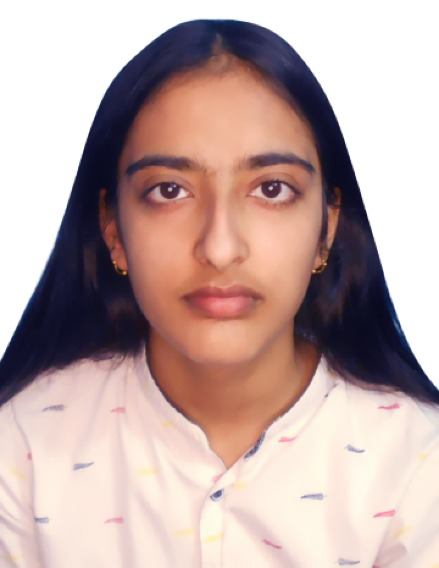
\includegraphics[width=3.0cm,height=1.5cm,keepaspectratio]{t.jpeg}
\end{minipage}
\\
\hline

\begin{minipage}[t][3.25cm][t]{\linewidth}
\vspace{1.5mm}
\textbf{Team member 2}\\[-1mm]
\textit{(Last Name, name: student ID: email, picture):}
\vspace{2.0cm}
\end{minipage}
&
\begin{minipage}[t][3.25cm][t]{\linewidth}
\vspace{1.5mm}
\footnotesize
\textit{Jahnavi -- 2510380066}\\
\textit{jahnavimittal89@gmail.com}

\vspace{2mm}
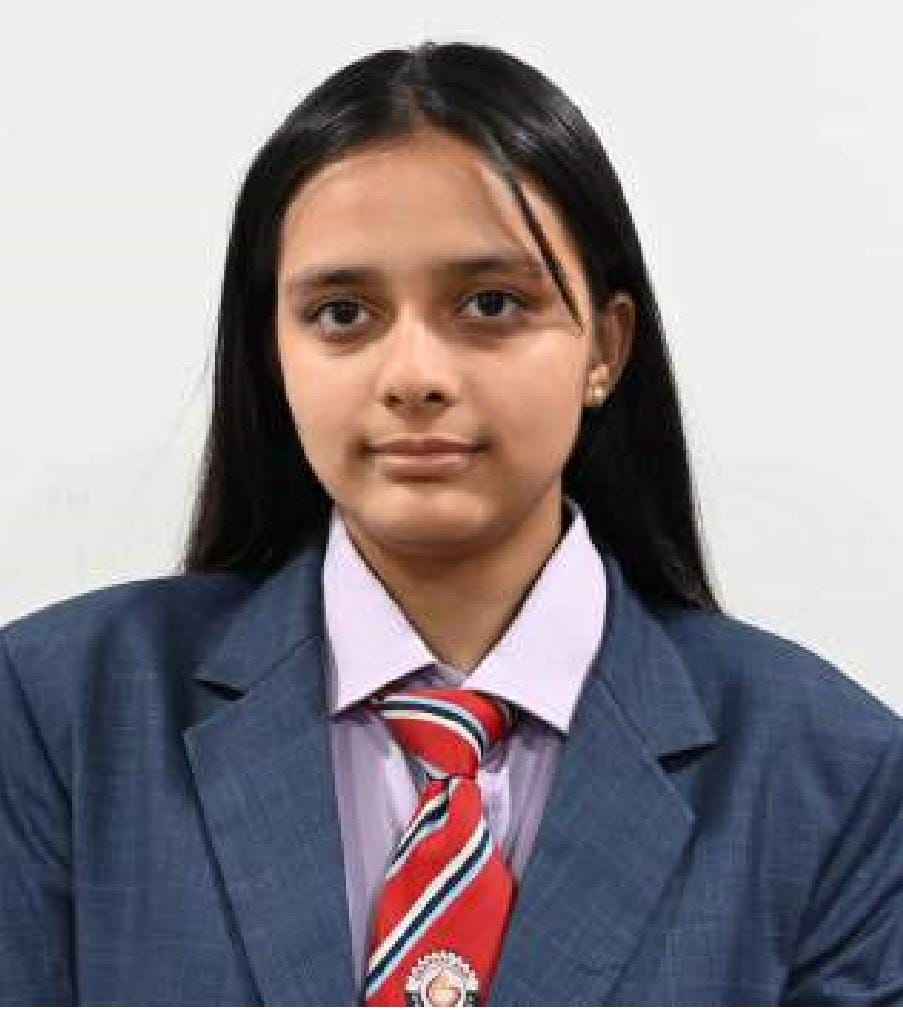
\includegraphics[width=3.0cm,height=1.5cm,keepaspectratio]{j.jpeg}
\end{minipage}
\\
\hline

\begin{minipage}[t][3.25cm][t]{\linewidth}
\vspace{1.5mm}
\textbf{Team member 3}\\[-1mm]
\textit{(Last Name, name: student ID: email, picture):}
\vspace{2.0cm}
\end{minipage}
&
\begin{minipage}[t][3.25cm][t]{\linewidth}
\vspace{1.5mm}
\footnotesize
\textit{Tyagi, Nishtha -- 2510370096}\\
\textit{nishthatyagii29@gmail.com}

\vspace{2mm}
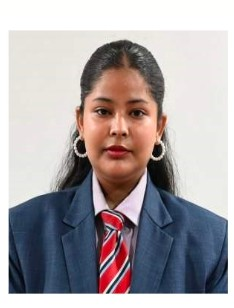
\includegraphics[width=3.0cm,height=1.5cm,keepaspectratio]{n .jpeg}
\end{minipage}
\\
\hline

\begin{minipage}[t][3.25cm][t]{\linewidth}
\vspace{1.5mm}
\textbf{Team member 4}\\[-1mm]
\textit{(Last Name, name: student ID: email, picture):}
\vspace{2.0cm}
\end{minipage}
&
\begin{minipage}[t][3.25cm][t]{\linewidth}
\vspace{1.5mm}
\footnotesize
\textit{Sharma, Dhairya -- 2510011490}\\
\textit{sharmadhairya820@gmail.com}

\vspace{2mm}
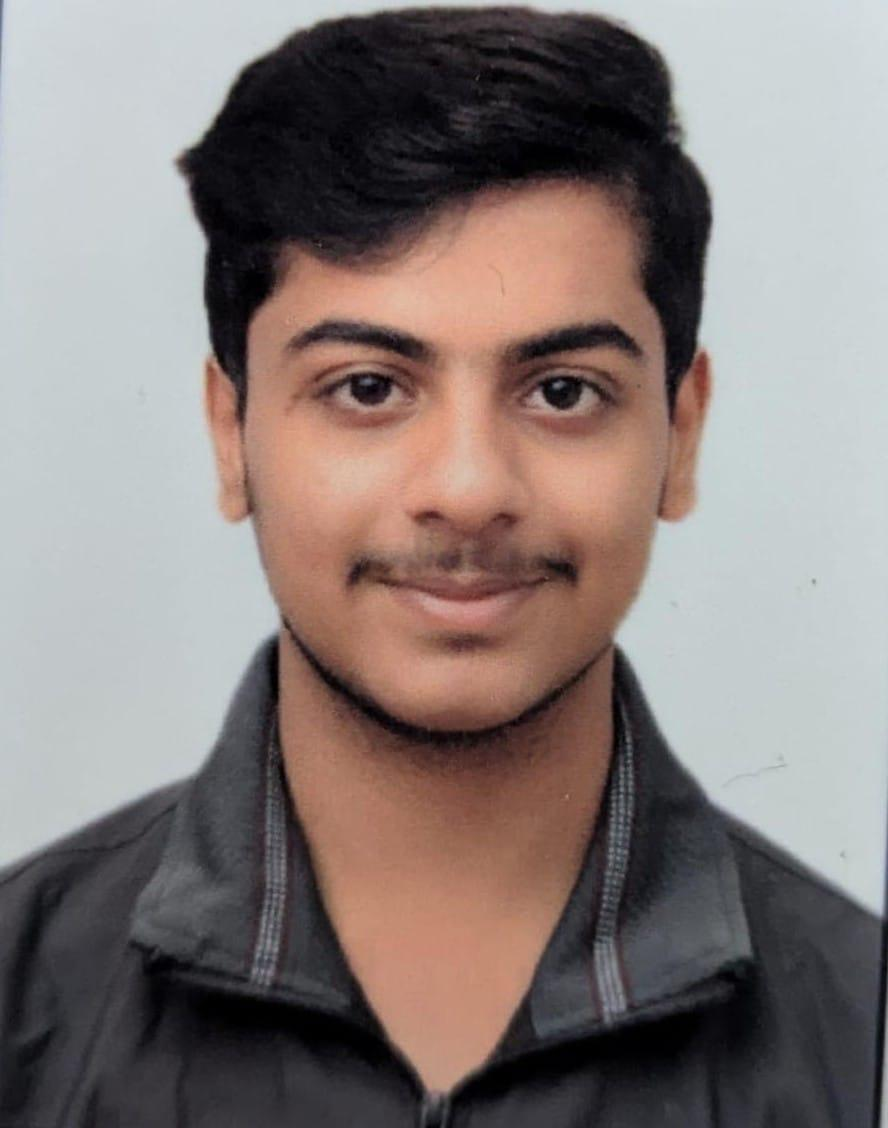
\includegraphics[width=3.0cm,height=1.5cm,keepaspectratio]{d.jpeg}
\end{minipage}
\\
\hline

\end{tabularx}

\vspace{0.45cm}

% ============================================================
% MENTOR INFORMATION
% ============================================================
\noindent
\begin{tabularx}{\textwidth}{
|>{\RaggedRight\arraybackslash}p{0.56\textwidth}
|>{\RaggedRight\arraybackslash}X|
}
\hline

\begin{minipage}[t]{\linewidth}
\vspace{2mm}
\textbf{Mentor Name:}\\[-1mm]
\textbf{Mentor Email Address:}
\vspace{2mm}
\end{minipage}
&
\begin{minipage}[t]{\linewidth}
\vspace{2mm}
\textit{Dr. Hemant Singh Pokhariya}\\
\textit{hemantsinghpokhariya@geu.ac.in}
\vspace{2mm}
\end{minipage}
\\
\hline

\end{tabularx}

\newpage

% ============================================================
% PAGE 2
% ============================================================

\vspace*{0.15cm}

\noindent
\colorbox{GEUBannerBlue}{%
\parbox{\dimexpr\textwidth-2\fboxsep\relax}{
    \vspace{0.18cm}
    {\color{GEUYellow}
    \fontsize{17}{21}\selectfont
    \bfseries
    PHASE-III PROJECT PROGRESS DESCRIPTION}
    \vspace{0.18cm}
}}

\vspace{0.70cm}

% PROJECT ABSTRACT
\sectiontitle{Project Abstract}

\vspace{0.05cm}

\vspace{0.12cm}

\answerbox{4.60cm}{
The main goal of our project, RideSync, is to build a comprehensive Smart Cab Booking and Dispatch Simulation System. Traditional cab allocation suffers from manual driver assignment, lack of real-time shortest-path route calculation, and inefficient dispatch mechanisms.

In Phase 3, we expanded RideSync from a purely C++17 console-based core engine into a full-stack interactive web platform. City locations and road connections are modeled as weighted graphs, and shortest routes are computed using Dijkstra's Algorithm. Driver selection is managed through a priority queue utilizing a composite scoring model (distance and driver rating). Data persistence is guaranteed through backend JSON storage and file logs, connecting a responsive frontend with a Node.js REST API server.
}

\vspace{0.70cm}

% UPDATED PROJECT APPROACH
\sectiontitle{Updated Project Approach and Architecture}

\vspace{0.05cm}

\vspace{0.25cm}

\answerbox{7.60cm}{
Our system features a dual-layer architecture: a core C++17 object-oriented algorithmic backend and a Node.js web application layer. The core C++ modules encompass \texttt{Customer}, \texttt{Driver}, \texttt{Admin}, \texttt{CityGraph}, and \texttt{BookingManager}. The road network of Dehradun is stored as an adjacency list using \texttt{std::unordered\_map<int, std::vector<std::pair<int, int>{}>{}>}. Shortest paths and minimum travel distances are calculated via Dijkstra's Algorithm with \texttt{std::priority\_queue}.

For driver dispatching, a max-heap priority queue evaluates candidates based on a composite score ($S = 0.7 \times \text{Rating} - 0.3 \times \text{Distance}$). STL containers (\texttt{vector}, \texttt{queue}, \texttt{priority\_queue}, \texttt{unordered\_map}, and a \texttt{stack} for recent booking history) optimize algorithmic execution.

To enhance accessibility, a modern responsive web interface (\texttt{HTML5}, \texttt{CSS3}, \texttt{JavaScript ES6}) was added along with a lightweight \texttt{Node.js} server (\texttt{server.js}). The frontend communicates via REST API requests to handle user login, real-time fare estimates, live booking dispatching, driver consoles, and administrative controls.
}

\newpage

% ============================================================
% PAGE 3
% ============================================================
\vspace*{0.20cm}

% TASKS COMPLETED
\sectiontitle{Tasks Completed}

\vspace{0.05cm}

\vspace{0.20cm}

\begin{tabularx}{\textwidth}{
|>{\RaggedRight\arraybackslash}X
|>{\RaggedRight\arraybackslash}p{0.28\textwidth}|
}
\hline

\textbf{Task Completed} &
\textbf{Team Member}\\
\hline

Problem definition, requirement analysis and overall system design (Phase 1) &
All team members \\
\hline

Object-oriented hierarchy (\texttt{User}, \texttt{Customer}, \texttt{Driver}, \texttt{Admin}) and C++ authentication module (\texttt{auth.cpp}) &
Tanvi Gupta \& Nishtha Tyagi \\
\hline

City map adjacency list representation (\texttt{graph.cpp}) and Dijkstra's shortest path routing algorithm &
Jahnavi \\
\hline

Driver priority queue dispatch engine (\texttt{dispatch.cpp}) using composite distance/rating scoring &
Dhairya Sharma \\
\hline

Booking lifecycle management, distance-based dynamic fare calculation, and C++ unit testing (\texttt{test\_core.cpp}) &
Tanvi Gupta \& Dhairya Sharma \\
\hline

Development of responsive Web UI (\texttt{index.html}, \texttt{style.css}, \texttt{app.js}) and Node.js backend REST server (\texttt{server.js}) &
Dhairya Sharma \& Tanvi Gupta \\
\hline

File handling persistence (\texttt{fstream} and JSON), system integration, end-to-end testing, and deployment setup &
All team members \\
\hline

\end{tabularx}

\vspace{0.65cm}

% CHALLENGES
\sectiontitle{Challenges/Roadblocks}

\vspace{0.05cm}

\vspace{0.18cm}

\answerbox{5.30cm}{
1. **Frontend-Backend Integration:** Synchronizing route calculations between the Node.js web server API endpoints and the underlying graph structures required careful API response structuring.

2. **Composite Score Calibration:** Fine-tuning weights in the driver priority queue ($0.7 \times \text{Rating} - 0.3 \times \text{Distance}$) to ensure optimal driver assignment without penalizing drivers slightly farther away.

3. **Data Persistence Alignment:** Ensuring seamless state synchronization between flat file storage in C++ and JSON storage (\texttt{ridesync.json}) on the Node.js server.

4. **Cross-Platform Compilation:** Managing build settings across standard C++17 toolchains (`Makefile`) and Node.js environment setups.
}

\vspace{0.65cm}

% TASKS PENDING
\sectiontitle{Tasks Pending}

\vspace{0.05cm}

\vspace{0.18cm}

\begin{tabularx}{\textwidth}{
|>{\RaggedRight\arraybackslash}X
|>{\RaggedRight\arraybackslash}p{0.34\textwidth}|
}
\hline

\textbf{Task Pending} &
\textbf{Team Member (to complete the task)} \\
\hline

None -- All project tasks, modules, web integrations, and testing milestones are 100\% completed. &
All team members \\
\hline

\end{tabularx}

\newpage
% ============================================================
% PAGE 4
% ============================================================

\vspace*{0.30cm}

% PROJECT OUTCOME
\sectiontitle{Project Outcome/Deliverables}

\vspace{0.05cm}

\vspace{0.35cm}

\answerbox{7.7cm}{
The project is fully completed and delivers a comprehensive multi-tiered system:

\begin{itemize}
\setlength{\itemsep}{0pt}
\setlength{\topsep}{2pt}
\item **Core C++17 Engine:** Fully functioning modular OOP implementation (\texttt{auth}, \texttt{graph}, \texttt{dispatch}, \texttt{system}).
\item **Graph Routing Engine:** Dijkstra's shortest path algorithm operating on city adjacency lists.
\item **Smart Dispatcher:** Max-heap priority queue matching drivers using composite scoring.
\item **Interactive Web Application:** Frontend interface providing customer booking, driver console, and admin dashboards.
\item **Node.js REST API Server:** Lightweight backend processing requests and serving location and booking endpoints.
\item **JSON \& File Persistence:** Storage layer maintaining system state across application restarts.
\item **Automated Core Tests:** C++ unit test executable (\texttt{test\_core.cpp}) validating algorithms.
\item **GitHub Repository:** Well-structured repository with complete source code, documentation, and commit history.
\end{itemize}
}

\vspace{0.75cm}

% PROGRESS OVERVIEW
\sectiontitle{Progress Overview}

\vspace{0.05cm}

\vspace{0.25cm}

\answerbox{5.00cm}{

Phase 1: Problem definition, requirement analysis, and system architecture design -- **COMPLETED**

Phase 2: Object-oriented class hierarchy, C++ authentication module, and core graph data structure setup -- **COMPLETED**

Phase 3: Implementation of Dijkstra's shortest path routing, driver dispatch priority queue, Node.js web server, and interactive Web UI -- **COMPLETED**

Phase 4: Data persistence integration, unit testing, and web interface polish -- **COMPLETED**

Phase 5: Final deployment, end-to-end testing, report compilation, and viva demonstration preparation -- **COMPLETED (100\%)**

}

\newpage

% ============================================================
% PAGE 5
% ============================================================

\vspace*{0.20cm}

% CODEBASE
% ---------- Codebase Information ----------
\vspace*{0.20cm}
\sectiontitle{Codebase Information}
\vspace{0.05cm}
\vspace{0.20cm}

\answerbox{9.0cm}{
\textbf{Repository link:} \texttt{github.com/TanviGupta12/RideSync-Cab-Booking-Dispatch}\\[3pt]
\textbf{Branch:} main\\[5pt]

Our team uses GitHub for version control and VS Code for development. Modules are logically separated into clean C++ header/source files alongside web application directories.\\[5pt]

\textbf{Important Commits}
\vspace{-3pt}

\begin{itemize}
    \setlength{\itemsep}{2pt}
    \setlength{\parskip}{0pt}
    \setlength{\topsep}{2pt}
    \setlength{\leftmargin}{15pt}
    \small

    \item \textbf{Tanvi Gupta:} Initialized project structure and base User/Customer/Driver class hierarchy.

    \item \textbf{Jahnavi:} Implemented \texttt{CityGraph} adjacency list and Dijkstra's shortest-path routing engine.

    \item \textbf{Nishtha Tyagi:} Added \texttt{std::stack}-based recent booking history tracking and customer profile management.

    \item \textbf{Dhairya Sharma:} Built \texttt{DriverPriorityQueue} dispatch logic and candidate scoring functions.

    \item \textbf{Tanvi Gupta:} Implemented distance-based dynamic fare calculator and \texttt{fstream} file persistence.

    \item \textbf{Dhairya Sharma:} Developed Node.js server (\texttt{server.js}) and REST API endpoints for web integration.

    \item \textbf{Dhairya Sharma \& Tanvi Gupta:} Designed responsive web interface (\texttt{index.html}, \texttt{style.css}, \texttt{app.js}).

    \item \textbf{Tanvi Gupta:} Integrated CLI entry point (\texttt{main.cpp}) and test suite (\texttt{test\_core.cpp}).
\end{itemize}
}

\vspace{0.35cm}

% TESTING
\sectiontitle{Testing and Validation Status}

\vspace{0.05cm}
\vspace{0.30cm}

\begin{tabularx}{\textwidth}{
|>{\RaggedRight\arraybackslash}p{0.30\textwidth}
|>{\RaggedRight\arraybackslash}p{0.22\textwidth}
|>{\RaggedRight\arraybackslash}X|
}
\hline

\textbf{Test Type} &
\textbf{Status (Pass/Fail)} &
\textbf{Notes}
\\
\hline

C++ Core Unit Testing (\texttt{test\_core.cpp})
&
PASSED
&
Verified Dijkstra routing, driver priority queue ranking, and user auth.
\\
\hline

Input Validation Testing
&
PASSED
&
Handled invalid location IDs, out-of-service drivers, and bad inputs gracefully.
\\
\hline

Web API \& Server Verification
&
PASSED
&
Tested authentication, route estimation, and ride booking endpoints on \texttt{localhost:3000}.
\\
\hline

Integration Testing
&
PASSED
&
Verified full flow across customer UI, server processing, and backend state persistence.
\\
\hline

\end{tabularx}

\vspace{0.65cm}

% DELIVERABLES PROGRESS
\sectiontitle{Deliverables Progress}

\vspace{0.05cm}

\vspace{0.25cm}

\answerbox{6.20cm}{
Customer, Driver, and Admin C++ Modules: Completed\\[2pt]
Shortest Path Route Engine (Dijkstra's Algorithm): Completed\\[2pt]
Priority-Queue Driver Dispatch System: Completed\\[2pt]
Dynamic Fare Calculation Engine: Completed\\[2pt]
Node.js REST API Server \& Web Interface: Completed\\[2pt]
JSON Data \& File Persistence: Completed\\[2pt]
Automated C++ Unit Test Suite: Completed\\[2pt]
Public Deployment \& Final Documentation: Completed
}

\end{document}